\chapter{Resultados}

\section{Resultados durante la fase exploratoria}

Inicialmente, tras finalizar el nivel o jugar durante 12 minutos, se pidió a usuarios expertos que evaluaran la usabilidad del juego en una escala del 1 al 10.

Se realizaron tres iteraciones utilizando esta metodología, junto con la recopilación de comentarios abiertos. En la primera fase, la usabilidad promedio entre 4 usuarios fue de 2.5.

Posteriormente, después de implementar las sugerencias previas, la usabilidad aumentó a 6 con una muestra de 4 usuarios. Sin embargo, los usuarios señalaron la facilidad para cometer errores y la monotonía del juego, así como la necesidad de leer mucho, lo cual generaba insatisfacción, a pesar de entender las acciones posibles.

Finalmente, antes de probar con el público objetivo, se llevó a cabo una última prueba con una muestra de 6 usuarios, obteniendo un promedio de calificación de 8 sobre 10. En este caso, los usuarios mencionaron problemas menores, principalmente relacionados con la interpretación de algunas animaciones o la falta de indicaciones, como la necesidad de presionar ENTER para avanzar en el código.

\section{Resultados de la fase de evaluación académica}

\subsection{Prueba académica}

Las 15 personas que hicieron la prueba tuvieron ambas respuestas correctas, identificando correctamente el recorrido BFS y DFS en cada caso. La prueba realizada se encuentra en el \hyperref[AnexoB]{anexo B}.

\subsection{Formulario MEEGA+: Percepción de usuario}

% Hablar de la suma de puntaje y puntaje promedio para los dos casos: De fase exploratoria y fase posterior.
% Poner acá gráficos y demás
Según \cite{meegaplus} un set de respuestas de un individuo se considera correcto y válido cuando tiene más del 85\% de las preguntas contestadas. En este caso no hubo omisiones.

En la figura \ref{RespuestasAgregadas} se muestran los resultados agregados para cada pregunta en cada categoría. Las preguntas se acortaron con acrónimos, pero la indexación está disponible en el \hyperref[AnexoA]{anexo A}.

\begin{figure}[h]
	\centering
	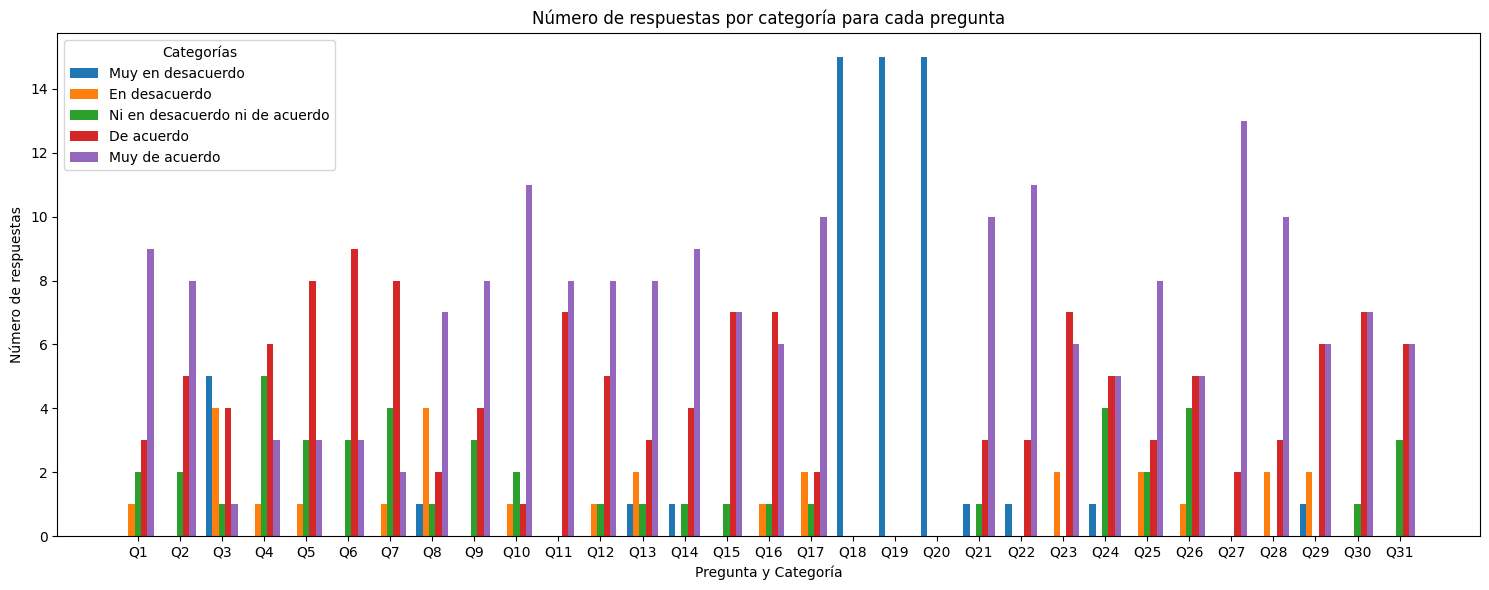
\includegraphics[scale=.45]{imagenes/answers.png}
	\caption{Agregación de respuestas por categoría y por pregunta}
	\label{RespuestasAgregadas}
\end{figure}

Por otra parte, en \cite{meegaplus} se utiliza Item Response Theory (IRT) para asignar un valor $\theta$ para la calidad del juego. Este se calcula a través de un script de R entregado en la \href{http://www.gqs.ufsc.br/quality-evaluation/meega-plus/}{\text{página del Software Quality Group de la Universidad Federal Santa Catarina de Brasil}} \cite{meegaplusQualityEvaluationPage}.

En tal página, se entrega un archivo de parámetros que pondera cada pregunta, además de asignar un valor de dificultad de elección entre cada item. Es decir, indica qué tan difícil es que un usuario se encuentre entre responder, por ejemplo, muy en desacuerdo y en desacuerdo, facilitando la distinción entre opiniones.

Aplicando el script en el \hyperref[AnexoE]{anexo E} con los parámetros entregados en la página con el manual de uso del modelo MEEGA+ \cite{meegaplusQualityEvaluationPage}, y las respuestas al formulario, se entrega un valor $\theta$ que indica la calidad del juego producido y permite clasificarlo. En este caso, el resultado obtenido fue de un $\theta = 0.613$, lo que significa que es un juego de buena calidad, mas no de excelente calidad según \cite{meegaplus}, pues para lograr la calidad excelente se requiere un valor $\theta \geq 0.65$.

En el anexo \hyperref[AnexoF]{Anexo F} se muestran los comentarios abiertos que se exigen en la metodología MEEGA+ \cite{meegaplus}.  

\section{Resultados de la encuesta libre}

Esta encuesta sigue libre al momento de la escritura de esta tesis. Hasta ahora, se han recolectado 11 respuestas. El resultado de la percepción con la metodología \cite{meegaplus} es un  $\theta = 0.616$. Los resultados se encuentran en los anexos de forma análoga a las respuestas posteriores. Se observa un valor $\theta$ más alto que en el caso anterior. Además, los comentarios abiertos muestran una actitud de mayor aceptación con respecto al grupo que se expuso a la prueba académica. Esto se puede deber al sesgo del voluntario \cite{volunterBias}, puesto que la comunidad que participó de este trabajo es una comunidad indie de creación de videojuegos, por lo que aprecian cada aspecto de los videojuegos y reconocen la dificutad de realizarlos.

Nuevamente, en el anexo \hyperref[AnexoF]{Anexo F} se muestran los comentarios abiertos que se exigen en la metodología MEEGA+ \cite{meegaplus}. Las respuestas están separadas con respecto al grupo anterior. 
